% Chapter 1

\chapter{Introduction} % Chapter title

\label{ch:introduction} % For referencing the chapter elsewhere, use \autoref{ch:introduction} 

%----------------------------------------------------------------------------------------

\emph{Multilevel security} (MLS) is a very popular term in security field. 
It either means a 'system' which delivers MLS as a service or it means an aspect of an existing system. 
Usually users (subjects in MLS genre) have different roles when dealing with files\dots (objects in MLS genre).
Subjects will have distinct security levels to access objects to perform their job-related tasks.
It is very trivial in military systems and the detailed explanation will be introduced shortly in \autoref{ch:background}.

Thinking about IT-related organizations, one can see there are many scenarios for working in an interacting systems, where many users with various roles (\eg\,developers, designers, project managers, customers etc.) work together sharing same data sources, this is typical \eg to serious military security projects.
While most of existing project management tools available in the market focus on productivity and accessibility of the project, some services \eg FreshDesk provides further data protection (authentication, data integrity etc.). However, not many projects realize how important it is to protect user data internally. In fact, many of data leaks happen inside the organization. MLS can cover strenuously those multi-role issues. It could be used as a skeleton for a PM tool to help us to have an advanced view about PM and innumerable assets around it which we will discuss later.

The goal of this project is to evaluate how complex it is to build up a MLS management system used in IT industry.
As the result, we are going to see the difficulty, limitation and solutions of building an MLS system and try to learn from that.
In a working solution, we may find various paths to reach the goal, and we will analyze them in order to understand deeper about MLS to pick out the best handling way.

In the beginning of this document, we are going to see how MTS can fit into PM tool, brief explanation about the use-cases, and how we are going to cover them in our tool.
\marginpar{Since it is 'hot' and I use it to 'cook' my thesis}At the moment, we will name this project \myProject.

%----------------------------------------------------------------------------------------

\section{The Use-Cases}
\label{ch:introduction:use_cases}
Let us have an example of a web project with its team members having various roles like these:
\begin{description}
\item[Developer] The builder of the project, who only care about: \emph{Sprint backlog}, \emph{coding tickets}, \emph{test cases}, \emph{Sprint review}, \emph{daily report}.
\item[Designer] They do not need to know about what happens on the back stage, they only need access right to: \emph{Sprint backlog}, \emph{pages list}, \emph{designing tickets}, \emph{design layouts}.
\item[Project Manager] They concern about: \emph{Product backlog}, \emph{Sprint backlog}, \emph{Sprint review}, \emph{daily report}, \emph{coding and designing tickets}.
\item[Customer] The one who pays bills, so they need to access to: \emph{Product backlog}, \emph{Sprint backlog}, \emph{Sprint review}.
\end{description}

So, as we can see, there are multiple roles played in a project by participants who require different data source for their work.
\marginpar{MLS advantage: protect data from multiple categories access} 
Some of them require a common piece of data and the others require special ones.
This is what we normally see in most of PM tools feature list.
Though, many of them do not have access control on those data sources.
Other subjects with non-relating roles can still observe the data as long as it is public (if the tool supports privacy mode for data sharing).

Now, let me push this example to another level. In the \emph{Sprint review}, there are some comments and evaluation by the project manager to \emph{developers} and \emph{designers}, or some customer feedbacks at the company level.
These pieces of information have nothing to do with the rest of the team, except the \emph{Project Manager} (\ie the appropriate person who need access to them).
The key point of this is that all of information concerned to the project should be kept in one place for convenience in tracking and making future plans.
\marginpar{MLS advantage: protect data from multiple level access}At the same time, we want to isolate it from persons with improper security level interacting within the same system.
Another advanced use-case is that, even in the same project, there may be some features that only need to be accessed by high level developers \eg\, security features, customer's private information (bank account...) etc.
\marginpar{MLS advantage: create a transparent working environemnt}So that, we can see how \emph{Multi Level Security} (MLS) is applicable in \emph{Project Management Tools}, and it can also help us to create a transparent working environment where people only receive what is essential to them to finish their job without suffering from \emph{finding a leaf in the forest}.
The usecase overview is illustrated in \autoref{fig:introduction:use_cases:usecase_diagram}.

\begin{figure}[bth]
\myfloatalign
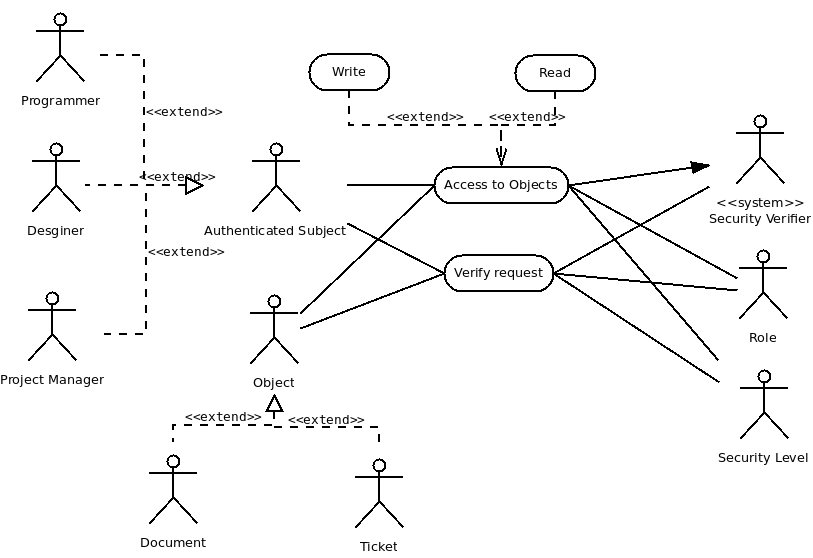
\includegraphics[width=1.0\linewidth]{gfx/chapter_1/usecase_diagram}
\caption[Usecase diagram]{Usecase diagram}\label{fig:introduction:use_cases:usecase_diagram}
\end{figure}

\section{Project Approach}
In \autoref{ch:background} , we will see in detail how MTS can implement this security feature.
In this section, I will introduce briefly about how we are going to design this program.

First of all, such as other MTS systems, we use things called \texttt{labels} (or \texttt{tag}).
Every subjects (\ie users) using the system will have one or many roles \eg\, developer, designer, or both etc., and they will be marked by one or many \emph{category labels}.
These labels are used to tell the system what kinds of document the subjects are interested in.
Moreover, in the same category, every subject should only have access to data which they need to know.
For example, a team leader, who is basically a senior developer, is the only one in the team should know about the customer's feedback, system changes, or customer's personal information etc...
even though those pieces of data can appear in a common directory (or even a file), they can only be viewed by the team leader.
\marginpar{\emph{Future plan}: read a document to intially evaluate its security level} 
We can control that by using another approach called \emph{security level label} \eg Top Secret, Secret, Authorised, Unauthorised etc...

So, basically, every subject in our system will have 2 kinds of label:
one or many \emph{category labels}, 
\marginpar{NOTE: may be one security level for every category labels} 
and \emph{ONLY} one \emph{security level label}.
And so does every data source.
They are nested together, using \emph{Bell--LaPadula} model,
to allow subjects to share and receive relevant data while restricting them from leaking data to extraneous ones,
and help people to save time to look for what they want.

Now, we have seen some use-cases of our project. 
They will be included as upcoming features, together with further security rules. 
In next chapter, we are going review about the history of MLS to understand more about how it solved real world problems and see how the others implemented it in their solutions.
